\documentclass[12pt,a4paper]{article}
\usepackage[utf8]{inputenc}
\usepackage{amsmath}
\usepackage{amsfonts}
\usepackage{amssymb}
\usepackage{makeidx}
\usepackage{graphicx}
\usepackage{lmodern}
\usepackage{url}
\usepackage{bm}
\usepackage{booktabs}
\usepackage{float}
\usepackage{caption}
\usepackage{subcaption}
\usepackage[left=2cm,right=2cm,top=2cm,bottom=2cm]{geometry}
\author{Mudathir Mahgoub}
\title{Project report}
\begin{document}

\maketitle

\section{Summary of the original project pitch}

The project proposal was titled Cozmo/Vector Uber which attempts to simulate Uber service with cozmo and vector robots. In this simulation, the robot world is a small map with roads where robots navigate around without a purpose, until some one requests a trip through the mobile app. Then the closest robot selected by the app would complete the trip by moving from the starting point to the destination. The app also  monitors trip status and displays robots movement on the map.  With this description, perhaps ``Robot Taxi" is a better name than ``Cozmo/Vector Uber" because Uber supports shared taxi which is beyond the scope of this project.

The project goals can be divided into 3 components described next. 

\subsection{Baseline goals for grade C} \label{sec:C}
The idea here is to implement the infrastructure needed for the simulation. The core of this infrastructure is a map, with roads and buildings, that is complex enough to support reasonable simulation. By reasonable simulation, I mean one that has multiple paths for the same trip to allow simple trip planning and shortest route computation. At the same time, the simulation doesn't need to be too complex to simulate every aspect of Uber which would be infeasible. It should be abstract enough to capture the main components of Uber service. After some thinking I settled on the map shown in figure \ref{fig:proposedMap}. To build that map, lego road plates and buildings were proposed. 
\begin{figure}[H]
\center
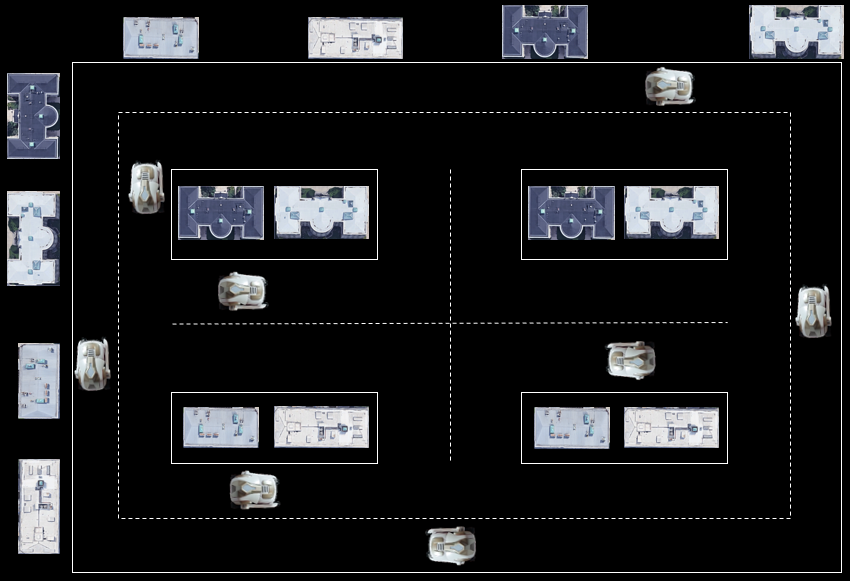
\includegraphics[scale=0.5]{./original_map.png}
\caption{The original proposed world.} \label{fig:proposedMap} 
\end{figure}


To implement the infrastructure for other components, the following goals were proposed: 

\begin{itemize}
\item Develop a server that assigns a new identifier to each connected robot client and monitors its current location.

\item Develop a robot client that connects to the server and periodically sends its status and current location to the server.

\item Develop a mobile app client which displays a map and the current locations of all robots connected to the server.
\end{itemize}
\subsection{Additional components for grade B} \label{sec:B}

After implementing the infrastructure, the next step is to support trips. To do that, the following goals  were proposed:

\begin{itemize}
\item Add the feature of trip requests to the mobile app which enables the user to specify the starting point and destination point on the map. Unlike the real world, in this world the mobile does not have a GPS to detect its current location. The user can specify the type of the robots: either spartan Cozmo or luxurious Vector. 

\item Add the trip planning feature to the server. For each trip request, the server identifies the nearest available robot and computes first the shortest route from the robot location to the  starting point, and then computes the shortest route from the starting point to the destination. The server then sends these routes to the selected robot.

\item Update the robot client to receive a trip plan and execute it.

\end{itemize}

\subsection{Top tier features for grade A} \label{sec:A}

To add some intelligence to the robot to avoid colliding with pedestrians and other robots,  the following goals were proposed:

\begin{itemize}
\item Build a neural network model to determine robot actions.
\item Process images taken by the camera. 
\item Stop all maneuvers if a person or a robot is detected to avoid collision. 
\end{itemize}

\section{Evaluation of project progress}
Here is the story of the project progress since the proposal. 
\subsection{Building the map}
The original proposal for the map included buildings which would make the simulation pretty fancy. However, after finding that the city buildings from Lego are too expensive, I moved them out of the project since they have little role in the implementation. Now that I am reflecting on the project, perhaps these buildings would help in the deep learning by stopping the robots from going outside the roads. The expenses could have been reduced if buildings were constructed from classical Lego small pieces and bricks. This can be done as future work, and I imagine kids would love to participate in constructing these buildings. 

For road plates I looked for square corners to simplify the navigation around corners. However, it seems Lego doesn't offer square corners, so  I settled for rounded corners which changed the map a little bit to look like figure \ref{fig:proposedMap}.

\begin{figure}[H]
\center
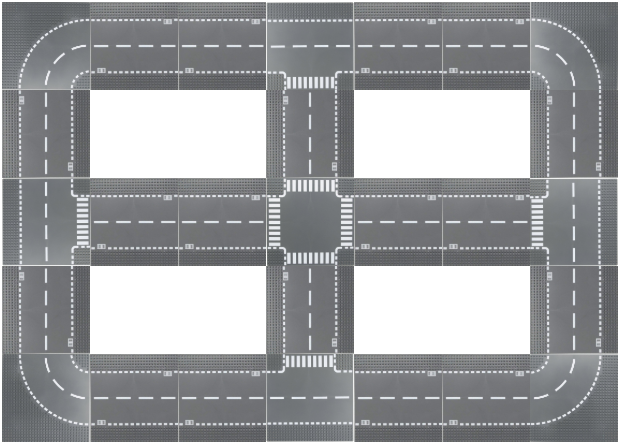
\includegraphics[scale=0.5]{./map.png}
\caption{The new world with empty white lands (without buildings).} \label{fig:proposedMap} 
\end{figure}

\subsection{Developing the server}
The next step after building the map is implementing the server. The server plays a central role in the project, and interacts with robots and mobile clients supporting different requests and responses. Therefore I chose Restful API approach with JSON to simplify the implementation. Since I was new to python, I looked for libraries that support Rest API and it seems Flask\footnote{\url{http://flask.pocoo.org/}} is a popular one. So I spent some time learning it and started implementing the server tasks. 

The first task was assigning a unique identity to each robot (which simulates Uber driver and car registration in real life). The first challenge was storing the ids of the robots. In real life, I imagine Uber storing the registration information in a secure database. Since security and persistence  are not concerns in this project, the database is overkill. So I preferred using a simple data structure in memory (dictionary in python) to act as a storage for robots information. The next challenge was a consequence of using a dictionary. Since no primary key restriction is forced in the dictionary data structure, multiple robots can get the same id if their requests arrive at the same time. So I followed the basic mutex synchronization by using the lock objects provided by the threading library in python. 


Now that the server can assign a unique id to each robot, what comes next is to determine what to store in the dictionary. So I created a new class named \textbf{RobotState}:(\textit{robot\_id, robot\_type, x, y, rotation, update\_time}) which would be updated later to include trip information. Then I created server methods that support getting and posting robot status, and created some unit tests to make sure they are working as expected. 

\subsection{Developing the mobile client}

Now that the server supports simple features, the next step is to implement one of the clients: either the mobile client or the robot client. I decided to implement the mobile client first, since it is faster and purely software. Implementing the mobile app first would also in understanding the requirements for the robot client. 

For the mobile app, I need to display the map, locations of connected robots, and animation for their movements. At first I thought of implementing the mobile app on android devices. But since many students use IPhone, cross platforms compatibility would be an issue.  Another issue was that cozmo already requires a mobile device, so I would need 2 android devices: one for cozmo, and one for the mobile app. This would make the development painful and unnecessary complicated. Fortunately,  the solution to such problems is straightforward: developing a web page which is accessible by web browsers in all platforms including mobile devices. So it was time to refresh my rusty knowledge about javascript language. 


The first challenge I encountered, is how to draw maps and animations on a web page. Back then, my  basic javascript knowledge  didn't include drawing. So it was time  to look for libraries specialized on that. The search result was D3\footnote{\url{https://d3js.org/}} which stands for Data-Driven Documents. Its gallery\footnote{\url{https://github.com/d3/d3/wiki/Gallery}} looks very exciting with graphs, maps and animation. To learn D3 I watched the online course \textit{d3-getting-started} from pluralsight\footnote{\textit{https://app.pluralsight.com/library/courses/d3-getting-started/table-of-contents}} to get started as its title says. After reading an article\footnote{\url{http://www.cagrimmett.com/til/2016/08/17/d3-lets-make-a-grid.html}} about drawing a grid using d3, I knew what to do and started coding. 


The first thing to draw was the map. To avoid hard coding the map, I created a Json file to store the map as cells. Each cell has the properties \textit{column, row, type, shape}. The cell type could be \textit{building} or \textit{road}. The shape of the building is not important and has no effect in the simulation. A road cell can have one of the following shapes: \textit{straightHorizontal, straightVertical, curveTopLeft, curveBottomLeft, curveBottomRigt, curveTopRight, tRight, tBottom, tLeft, tTop} and \textit{cross}.

Since web pages can't access files in the client machine, I made a special API for the map in the server so that the web page can retrieve the map when page content is loaded. When the map reaches the web client, each cell gets drawn according to its type and shape as shown in figure \ref{fig:proposedMap}. The next step is drawing some robots. 

\subsection{Developing the robot mock client}

After displaying the map on the web client, it is natural to implement cozmo client next. However I was reluctant to do that immediately for two reasons. First I have only one cozmo, so I would only see one robot on the map if I implemented it first. Second cozmo development needs more time and configuration because it has hardware components and needs charging. So a \textit{mock client} that is purely software, simulates cozmo, doesn't need charging,  and requires only the desktop sounded very reasonable. 

Initially I ran multiple mock clients at once without movement. The web client displayed them correctly but it wasn't fun because no animation was involved. To do animation I had to implement random movements for the robot based on their current location. Since d3 uses CSS transitions for animation, I didn't need to implement movements on the pixel level. The cell level (which is 80 pixel) was enough for d3 to do its magic. So all I needed is to move the mock robot from one road cell to a neighbor cell. Since backward movements and U-turns are not supported, the robot has at most 3 options depending on shape of its current cell: \textit{go straight}, \textit{turn right} or \textit{turn left}. 

For simplicity the mock client supports only 4 rotations: \textit{down} with rotation angle 0, \textit{up} with rotation angle 180, \textit{right} with rotation angle 90, and \textit{left} with rotation \textit{-90}. A challenge related to rotations was displaying them correctly using d3. Only \textit{down} rotation works perfectly. Other rotations are little off and it seems their geometric calculations need revisiting. With this, I thought I know what need to be done with the real client (cozmo client). How naive I was is described next. 

\subsection{Developing the cozmo client} \label{sec:failures}

Like the mock client, the plan for the cozmo client is to determine its current cell, randomly choose one of its neighbors, and choose the appropriate motor actions. However, I encountered a big problem: determining the current cell based on the position returned by cozmo  API was not accurate. 

It was really frustrating trying to navigate cozmo correctly on the map. First I tried controlling its wheels based on its positions, but that failed miserably. Then I tried computing the position myself following discrete movements to avoid positioning methods from cozmo API as follows:
\begin{itemize}
\item Start with \textit{current position} $=(x, y, rotation) = (0, 0, 0)$.
\item Use discrete actions to move cozmo to the next cell based on \textit{current position} which determines the \textit{current cell}. An example: 
\begin{enumerate}
\item $drive\_straight(distance)$
\item $turn\_in\_place(angle)$
\end{enumerate}

\item Update \textit{current cell} after completing the actions. After executing the above actions the \textit{current position} would be $(x, y, rotation) = (distance, 0, angle)$
\end{itemize}

This second approach also failed because  $turn\_in\_place(angle)$ was not reliable. I was stuck at this point, so I postponed cozmo client and decided to do other things in the project. Since section \ref{sec:B} depends on cozmo client, I skipped it and focused on achieving the goals in section \ref{sec:A}. 

\subsection{Deep learning}
Using deep learning in an application was something new to me. So I asked around and people suggested using 
 TensorFlow\footnote{\url{https://www.tensorflow.org/}} library for python. After many attempts, I wasn't able to successfully install TensorFlow in my Windows machine. People suggested to me to use Anaconda platform\footnote{https://www.anaconda.com/distribution} to install python packages including TensorFlow. That also didn't work in Windows. So I gave up on using TensorFlow and decided to check deep learning in Matlab, an environment I am familiar with. 
 
It turned out that Matlab has a really nice deep learning framework and comes with  a nice GUI called Deep learning Network analyzer. After following their get-started tutorial\footnote{https://www.mathworks.com/help/deeplearning/gs/get-started-with-deep-network-designer.html}, I found that all I need to do is to put the training images in labeled folders and specify the number of classes to Matlab and then let it handle the rest. Matlab deep learning framework automatically figures out GPU support, displays training progress, and outputs the result into a variable in the workspace.  It was really nice experience compared to TensorFlow. 


Next I took some sample images with cozmo to try Matlab deep learning. After training was finished, I looked on how to import the trained models from Matlab into python. There is an open neural network exchange format called ONNX\footnote{\url{https://onnx.ai}} which is supported by TensorFlow, Matlab, and other deep learning frameworks. To install onnx for python, it requires a C++ library called Protobuf\footnote{\url{https://github.com/protocolbuffers/protobuf}}. After many attempts, I failed to successfully install onnx. So
I gave up on onnx and decided to use only Matlab and python. 

It turned out Matlab comes with python engine support\footnote{\url{https://www.mathworks.com/help/matlab/matlab_external/get-started-with-matlab-engine-for-python.html}} which enables python to connect to Matlab and call its functions and scripts. After installing this python engine\footnote{\url{https://www.mathworks.com/help/matlab/matlab_external/install-the-matlab-engine-for-python.html}} there are 2 options to connect to Matlab: starting a new session from python which waits until a new Matlab session is started, or sharing an existing session. I found that sharing an an already opened Matlab is more convenient, because it is instantaneous and I can see the workspace used by python. Now the deep learning environment is ready for cozmo.  

After playing with small number of images taken by cozmo, I thought of using deep learning to solve the issues I encountered in section \ref{sec:failures}. Since I need only 3 movement actions \textit{go-stright, turn-left, turn-right}, I can take images related to these 3 classes. After doing that the results were really promising that I totally changed my approach to cozmo client. Instead of trying to compute the next action based on the current cell, let the deep learning handle that. I started seriously taking a lot of training images and classified them into 9 classes: 
\textit{corner-left,
corner-right,
cross,
stop,
straight,
turn-left-left,
turn-left,
turn-right-right,\text{ and}
turn-right}. The \textit{stop} class includes images where cozmo sees the rear or the front of vector, and hence the action to avoid collision is to \textit{stop}. These classes didn't consider what to do in T cells (\textit{tLeft, tRight, tBottom, tTop}) and the \textit{cross} cell. 

At this point, the server had no clue about deep learning which is totally implemented in cozmo client. This is the right decision because in a real self-driving car, you don't want the decisions to be handled remotely by a server when you can lose connection at any moment. However, the project update presentation was coming and I wanted to try multiple cozmos on the map. I couldn't ask colleagues to install Matlab just for my presentation. So I moved the deep learning part to the server, and made cozmo client sends images to the server and receives their classifications. I was worried about the delay, but it wasn't bad after reducing the speed of cozmo wheels to 50 millimeters per second.  
 
In the project update presentation, the instructor provided 2 cozmo robots and we managed to connect them to the server. But the results were mixed, sometimes the robots move on-track and sometimes off-track. Sometimes cozmo collides with other robots and sometimes it stops. I was surprised that classification works well with cozmo seeing other cozmo, even though I trained images only with cozmo seeing vector. 

The instructor suggested many ideas to improve the navigation. One idea is installing bumpers to keep cozmo inside its lane. Another one is putting stickers on lego plates to help the image recognition. A third idea is simplifying roads and make them one-way instead of two-way. I preferred the third because it seemed the easiest one. However because of time constraint, I didn't have enough training images to get good performance on one-way roads. So I continued with two-way. 
 

\subsection{Trips}

So far in this project, I worked in achieving goals in section \ref{sec:C} and \ref{sec:A} and I didn't work in trips which are mentioned in section \ref{sec:B}. Since trip requests are initiated by the mobile client. I started with modifying the web client to allow users to select the starting point of the trip, the destination, and the preferred robot which is either \textit{cozmo} or \textit{vector}. Figure \ref{fig:tripRequest} shows an example of a trip request. 

\begin{figure}[H]
\center
\includegraphics[scale=0.5]{./tripRequest.png}
\caption{Example of a trip request.} \label{fig:tripRequest}
\end{figure}

A challenge I encountered in d3 is dynamically changing the images inside svg element (Scalable Vector Graphics). To solve this challenge, I added 2 layers of images: one for starting points, and another for destination points. Each layer contains a hidden image in each cell. When a cell is clicked, the appropriate image is displayed or hidden. Figure \ref{fig:layers} shows these 2 layers separately, but actually the destination layer is exactly above the start layer. 
\begin{figure}[H]
     \center
     \begin{subfigure}[b]{0.45\textwidth}
         \centering
         \includegraphics[width=\textwidth]{./startLayer}
         \caption{Starting points layer}
     \end{subfigure}
     \hfill
     \begin{subfigure}[b]{0.45\textwidth}
         \centering
         \includegraphics[width=\textwidth]{./destinationLayer}
         \caption{Destination points layer}
     \end{subfigure}
     \caption{Trip layers.}
     \label{fig:layers}
\end{figure}



As usual, I started with the mock client to implement trips. By default mock clients navigate randomly on the map. When a trip request is made, the server searches for ``nearest" robot to the starting point that matches the robot type in the request. The ``nearest" robot is defined as the one with the minimum  Manhattan distance  which is defined as :
\begin{align*}
distance( \langle row_2, column_2\rangle, \langle row_2, column_2 \rangle) = \vert row_2 - row_1 \vert +  \vert column_2 - column_2 \vert
\end{align*}

After nearest robot is selected, it receives the trip information from the server (\textit{status,  start.row, start.column,  end.row, end.column, robot\_type}). Trip \textit{status} can be: \textit{requested, waiting, started, or finished}. The initial value is \textit{requested} when the trip request is made. When the nearest robot is selected, the status is changed to \textit{waiting} and a green flag is attached to the selected robot. When the robot reaches the starting cell, the state is changed to \textit{started} and a red flag is attached to the robot. When the robot arrives to the destination, the status is changed to \textit{finished} and its flag is removed to indicate that the robot is available to  serve other trips. Figure \ref{fig:status} shows the flags that are attached to booked robots.

\begin{figure}
\center
\includegraphics[scale=0.5]{./tripStatus.png}
\caption{Trip status.} \label{fig:status}
\end{figure}

The mock client employs a simple algorithm to fulfill a trip request. When the mock client arrives to a cell with turns \textit{tLeft, tRight, tTop, tBottom, or cross}, it selects the cell with the minimum Manhattan distance to the starting point. After arriving to the starting point, it does the same for the destination. 
It should be noted this is not the best approach with the shortest route, but I am satisfied with it for the purpose of this project. A better approach wouldn't consider the starting point and destination separately, but would consider them together to reduce the total distance covered by the robot to complete the trip. With the current implementation, it may happen that the destination is close to the starting point, but the robot follows a longer route because U-turns are not supported in this project. 

\subsection{Trips and robot client}

So far cozmo client did not consider turning in cells \textit{tLeft, tRight, tBottom, tTop, cross}. But with trips, they need to be supported. So I tried to train cozmo to detect these cells. the T cells proved difficult because when cozmo is on a T cell and it is moving without turning, its camera may not see the current T cell. It is possible to detect this cell if cozmo is far enough or it turns towards the crosswalk on the T-cell. Both approaches are not easy since the former needs time synchronization, and the second disrupts the current movement. 

I tried a different approach, that combines image classification and positioning API from cozmo. Again I am using positioning methods from Cozmo API to know its current cell. As long as the robot is on a straight cell \textit{vertical or horizontal}, it uses only image classification. When it arrives to one of the cells \textit{tLeft, tRight, tBottom, tTop, cross}, then I ignore the image classification and move to one of the neighboring cells either randomly or  based on Manhattan distance to a target in a trip.  This approach didn't work well and suffered just like other approaches because positioning methods are not that reliable. At this point, I am convinced that the stickers option (figure \ref{fig:stickers}) suggested by the instructor could solve this problem. This is left as future work. 

\begin{figure}[H]
\center
\includegraphics[scale=0.3]{./stickers.jpg}
\caption{Stickers that can help cozmo in detecting the current cell.}
\label{fig:stickers}
\end{figure}


\subsection{Developing the vector client} 

There is no much difference between cozmo and vector in terms of API. However, vector images are colored and therefore I changed them to gray (black and white) in order to use cozmo trained model. This approach didn't work well, and I guess separate training images for vector may be needed. 
For presentation, working with vector is more difficult than cozmo because it needs some configuration with the WiFi, and its IP address needs to be configured each time it gets a new one. Nonetheless vector is more powerful and its movement is more stable, so finishing the vector client is left as future work. 

\subsection{Detecting pedestrians}

Section \ref{sec:A} mentions detecting pedestrians. I didn't buy a Lego person until the end of the project. So the trained model didn't include pedestrian images. Nonetheless during presentation with the instructor, cozmo actually stopped when a Lego person was put in front of it. However, few moments later, it had no problem hitting this person. So cozmo needs to learn about driving laws by reading more images which is left as future work. 

\section{Technical details} \label{sec:technical}

Here are the instructions to download and run the project:

\begin{enumerate}
\item Install python 3\footnote{Tested on 3.7} \url{https://www.python.org/downloads/}.
\item Install Cozmo SDK 
\begin{verbatim}
pip3 install  cozmo[camera]
\end{verbatim}
To upgrade a previous version run 
\begin{verbatim}
pip3 install --upgrade cozmo
\end{verbatim}
\item Install Flask Library required by server.py
\begin{verbatim}
pip3 install Flask
\end{verbatim}
\item Install requests library needed by clients
\begin{verbatim}
pip3 install requests
\end{verbatim}

\item Install Matlab 2019a or later versions \url{https://www.mathworks.com}.
\item Install MATLAB Engine API for Python\footnote{\url{https://www.mathworks.com/help/matlab/matlab_external/install-the-matlab-engine-for-python.html}}
\begin{verbatim}
cd "C:\Program Files\MATLAB\R2019a\extern\engines\python"
python setup.py install
\end{verbatim}
\item Download or clone the project RobotTaxi:
\begin{verbatim}
git clone https://github.com/mudathirmahgoub/RobotTaxi
\end{verbatim}
\item Run Matlab and navigate to the matlab folder in the project by running the command below in Matlab
\begin{verbatim}
cd 'C:\RobotTaxi\matlab'
\end{verbatim}

\item Load the workspace that contains the trained model by running the command below in Matlab 
\begin{verbatim}
load('matlab.mat')
\end{verbatim}
\item Make the current Matlab session shared by executing the command below
\begin{verbatim}
matlab.engine.shareEngine('DeepLearning')
\end{verbatim}

\item Run the server.py 
\begin{verbatim}
python server.py
\end{verbatim}

\item Now the server is running, you can browse the web client using the server IP address. For example \url{http://192.168.0.12:7000/app/trip.html}
\item You can now run the mock client and  pass either \textit{cozmo} or \textit{vector} as an argument which determines the robot type
\begin{verbatim}
python mock_client.py cozmo
python mock_client.py vector
\end{verbatim}

\item To run cozmo client, put Lego road plates as shown in the figure \ref{fig:zero} below. The starting cell for cozmo is shown as well which specifies the initial position for cozmo. $(x, y, rotation) = (0,0, 0)$. The initial cell is configurable and can be changed in file \textit{map.json} where \textit{startRow}  and \textit{startColumn} specify the initial cell.
\begin{verbatim}
python cozmo_client.py
\end{verbatim}

\begin{figure}[H]
\center
\includegraphics[scale=0.4]{./zero.png}
\caption{Initial position for cozmo. } \label{fig:zero}
\end{figure}


\item To take training images for cozmo and vector run the following files
\begin{verbatim}
python training_images_cozmo.py
python training_images_vector.py
\end{verbatim}

You need to modify the file to change the number of images, the directory and the image class

\begin{verbatim}
number_of_images = 5  # total number of the same image
directory = 'matlab/training_images/cozmo'  # directory for training images
image_class = 'turn-left'  # the image class or label
\end{verbatim}

\item To train the model in Matlab, update the line below in file ``create\_network.mlx". You just need to specify the number of classes in your model. In the line below, they are 7. 
\footnotesize
\begin{verbatim}
 fullyConnectedLayer(7,"Name","fc","BiasLearnRateFactor",10,"WeightLearnRateFactor",10)
\end{verbatim}
\normalsize
Then run the the following command to train the model 
\begin{verbatim}
run('train_network.m')
\end{verbatim}
Finally to save the trained model, save the workspace into a mat file by pressing ``ctrl+s".
\end{enumerate}

\section{Programming details}

The source code of this project is available in github \url{https://github.com/mudathirmahgoub/RobotTaxi}. It is written using programming languages python, javascript and Matlab. The web client source code is located in the directory \textit{app}. Matlab code is located in the directory \textit{matlab}. 
See section \ref{sec:technical} to run the project. 

\section{Acknowledgements and Gratitude}

I appreciate the instructor help  with the idea of this project, and how to tackle many problems arose during its development. I followed the quick start from Flask \url{http://flask.pocoo.org/docs/1.0/quickstart/} in building the server code. I learned d3 from this online course by Chris Behrens \\ \url{https://app.pluralsight.com/library/courses/d3-getting-started/table-of-contents}. I benefited  from a blog named ``Let's Make a Grid with D3.js" by Chuck Grimmett \url{http://www.cagrimmett.com/til/2016/08/17/d3-lets-make-a-grid.html} which helped me in drawing the map and trip requests. The deep learning part is based on a tutorial named ``Get Started with Deep Network Designer" from Matlab \url{https://www.mathworks.com/help/deeplearning/gs/get-started-with-deep-network-designer.html}. I got the idea of how to take images from this github project by Charlie Harrington \url{https://github.com/whatrocks/cozmo-tensorflow/blob/master/cozmo-paparazzi.py}. The cozmo client takes images following the camera example in the class github repository \url{https://github.com/CozmoRobots/Camera}. 

I also appreciate the help from the community of stackoverflow where I find the answers to many errors I encountered. 


\bibliographystyle{plain}

\bibliography{references}

\end{document}
